\documentclass[border=18pt]{standalone}
\usepackage[T1]{fontenc}
\usepackage[utf8]{inputenc}
\usepackage{circuitikz}
\usepackage{amsmath,amssymb}
\usetikzlibrary{positioning,calc}
\ctikzset{bipoles/length=1.15cm, font=\small}

\definecolor{tinta}{HTML}{1E293B}
\definecolor{ambar}{HTML}{C2410C}
\definecolor{azul}{HTML}{0E7490}
\definecolor{verde}{HTML}{15803D}
\definecolor{rojo}{HTML}{B91C1C}
\definecolor{gris}{HTML}{6B7280}
\definecolor{panel}{HTML}{F1F5F9}

\begin{document}
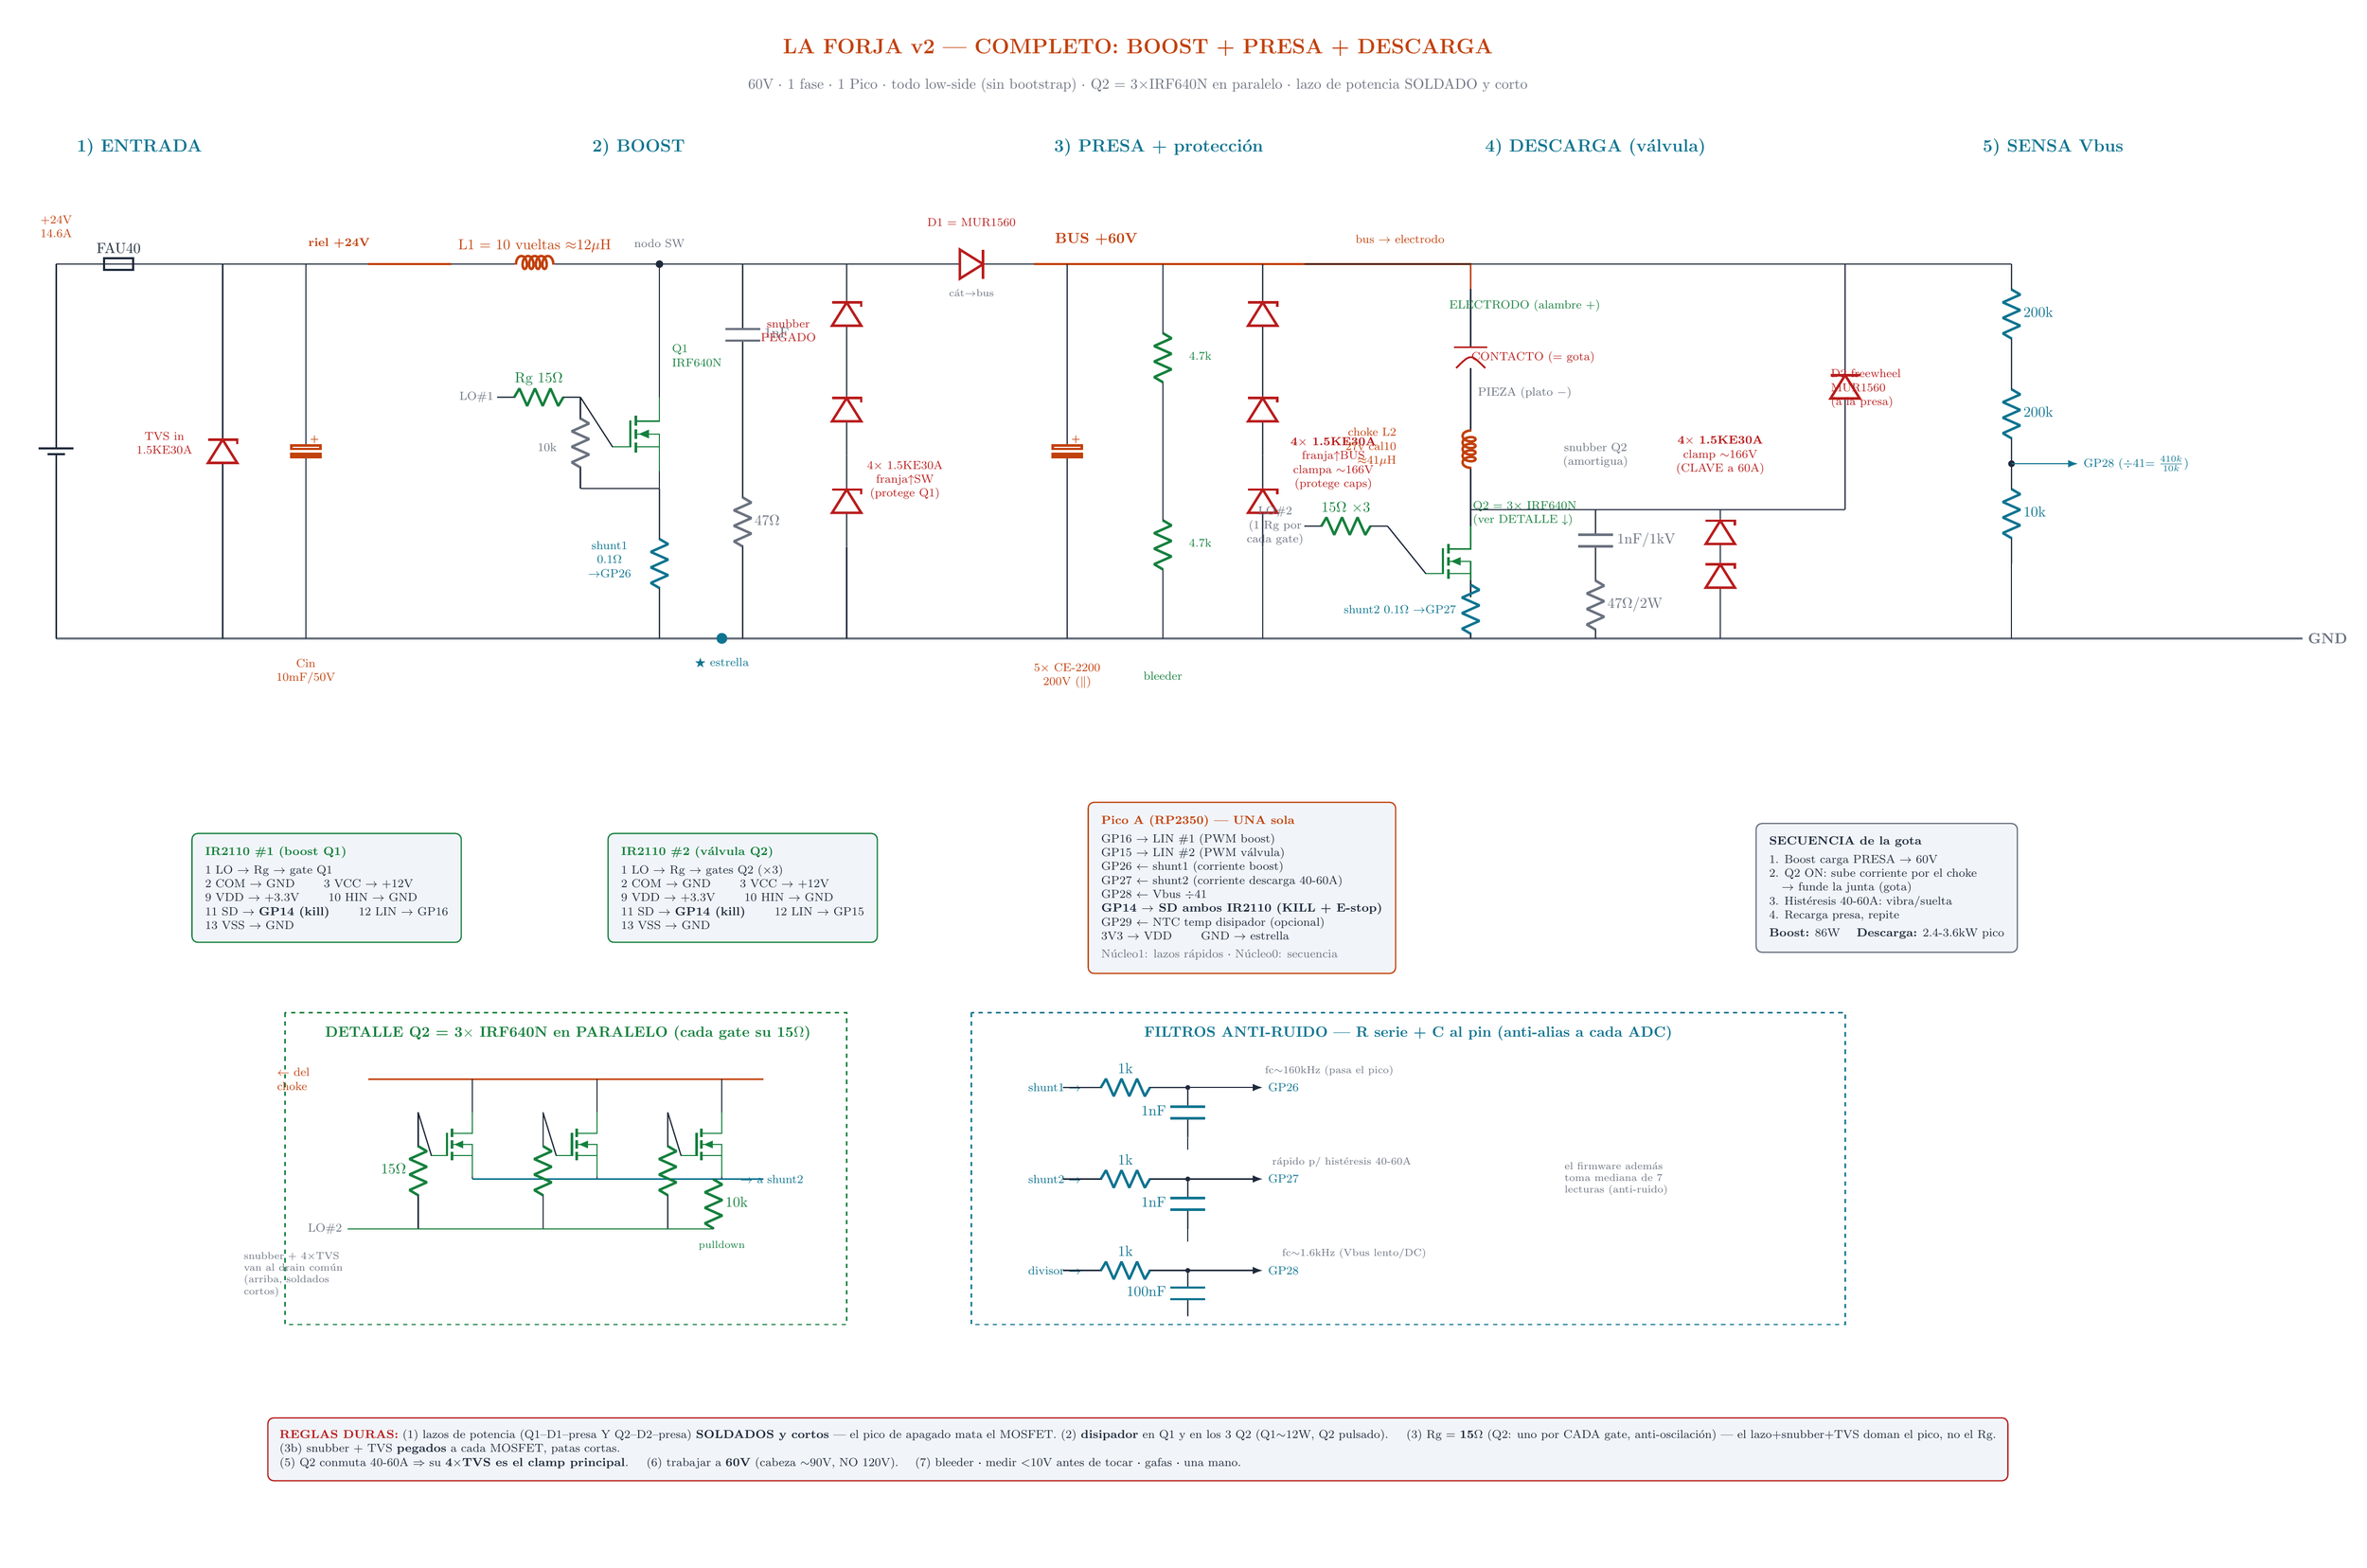
\begin{tikzpicture}[color=tinta, every node/.style={text=tinta}, line width=0.85pt]
\fill[white] (-11,-31) rectangle (45,6);

% ===== TITULO =====
\node[text=ambar, font=\bfseries\Large] at (16,5.2) {LA FORJA v2 — COMPLETO: BOOST + PRESA + DESCARGA};
\node[text=gris, font=\normalsize] at (16,4.3) {60V · 1 fase · 1 Pico · todo low-side (sin bootstrap) · Q2 = 3$\times$IRF640N en paralelo · lazo de potencia SOLDADO y corto};

% ===== RIEL GND =====
\draw[gris, line width=1.4pt] (-10,-9) -- (44,-9);
\node[text=gris, font=\bfseries] at (44.6,-9){GND};
\fill[azul] (6,-9) circle (0.13); \node[text=azul, font=\footnotesize] at (6,-9.6){$\bigstar$ estrella};

% ========================= 1) ENTRADA =========================
\node[text=azul, font=\bfseries\large] at (-8,2.8){1) ENTRADA};
\draw (-10,0) to[battery1] (-10,-9);
\node[text=ambar, font=\footnotesize, align=center] at (-10,0.9){+24V\\14.6A};
\draw (-10,0) to[fuse, l=\textcolor{tinta}{FAU40}] (-7,0);
\draw (-7,0) -- (-2.5,0);
\draw (-6,0) to[empty Zener diode, invert, color=rojo] (-6,-9);
\node[text=rojo, font=\footnotesize, align=center] at (-7.4,-4.3){TVS in\\1.5KE30A};
\draw (-4,0) to[ecapacitor, color=ambar] (-4,-9);
\node[text=ambar, font=\footnotesize, align=center] at (-4,-9.8){Cin\\10mF/50V};
\draw[ambar, line width=1.2pt] (-2.5,0) -- (-0.5,0);
\node[text=ambar, font=\bfseries\footnotesize] at (-3.2,0.5){riel +24V};

% ========================= 2) BOOST =========================
\node[text=azul, font=\bfseries\large] at (4,2.8){2) BOOST};
\draw (-0.5,0) to[L, l=\textcolor{ambar}{L1 = 10 vueltas $\approx$12$\mu$H}, color=ambar] (3.5,0);
\draw (3.5,0) -- (10.5,0); \fill[tinta] (4.5,0) circle (0.09);
\node[font=\footnotesize, text=gris] at (4.5,0.5){nodo SW};
% Q1 low-side
\node[nigfete, anchor=D, color=verde, scale=1.15] (Q1) at (4.5,-3.2){};
\draw (4.5,0) -- (Q1.D);
\node[text=verde, font=\footnotesize, align=left] at (5.4,-2.2){Q1\\IRF640N};
\draw (Q1.G) -- (2.6,-3.2);
\draw (2.6,-3.2) to[R, l_=\textcolor{verde}{Rg 15$\Omega$}, color=verde] (0.6,-3.2);
\node[font=\footnotesize, text=gris] at (0.1,-3.2){LO\#1};
\draw (2.6,-3.2) to[R, color=gris] (2.6,-5.4); \node[text=gris,font=\footnotesize] at (1.8,-4.4){10k};
\draw (2.6,-5.4) -- (4.5,-5.4);
\draw (Q1.S) -- (4.5,-5.4);
\draw (4.5,-5.4) to[R, color=azul] (4.5,-9);
\node[text=azul, font=\footnotesize, align=center] at (3.3,-7.1){shunt1\\0.1$\Omega$\\$\to$GP26};
% snubber Q1
\draw (6.5,0) to[C, l=\textcolor{gris}{1nF}, color=gris] (6.5,-3.4);
\draw (6.5,-3.4) to[R, l=\textcolor{gris}{47$\Omega$}, color=gris] (6.5,-9);
\node[text=rojo, font=\footnotesize, align=center] at (7.6,-1.6){snubber\\PEGADO};
% 4x TVS drain Q1
\draw (9,0) to[empty Zener diode, invert, color=rojo] (9,-2.4);
\draw (9,-2.4) to[empty Zener diode, invert, color=rojo] (9,-4.6);
\draw (9,-4.6) to[empty Zener diode, invert, color=rojo] (9,-6.8);
\draw (9,-6.8) -- (9,-9);
\node[text=rojo, font=\footnotesize, align=center] at (10.4,-5.2){4$\times$ 1.5KE30A\\franja$\uparrow$SW\\(protege Q1)};
% D1 al bus  -- etiqueta ARRIBA, despejada
\draw (10.5,0) to[D, color=rojo] (13.5,0);
\node[text=rojo, font=\footnotesize] at (12,1.0){D1 = MUR1560};
\node[text=gris,font=\scriptsize] at (12,-0.7){cát$\to$bus};

% ========================= 3) PRESA =========================
\node[text=azul, font=\bfseries\large] at (16.5,2.8){3) PRESA + protección};
\draw[ambar, line width=1.2pt] (13.5,0) -- (20,0);
\node[text=ambar, font=\bfseries] at (15,0.6){BUS +60V};
\draw (14.3,0) to[ecapacitor, color=ambar] (14.3,-9);
\node[text=ambar, font=\footnotesize, align=center] at (14.3,-9.9){5$\times$ CE-2200\\200V ($\parallel$)};
\draw (16.6,0) to[R, color=verde] (16.6,-4.5);
\draw (16.6,-4.5) to[R, color=verde] (16.6,-9);
\node[text=verde, font=\footnotesize] at (17.5,-2.2){4.7k}; \node[text=verde, font=\footnotesize] at (17.5,-6.7){4.7k};
\node[text=verde, font=\footnotesize] at (16.6,-9.9){bleeder};
% TVS DEL BUS
\draw (19,0) to[empty Zener diode, invert, color=rojo] (19,-2.4);
\draw (19,-2.4) to[empty Zener diode, invert, color=rojo] (19,-4.6);
\draw (19,-4.6) to[empty Zener diode, invert, color=rojo] (19,-6.8);
\draw (19,-6.8) -- (19,-9);
\node[text=rojo, font=\footnotesize, align=center] at (20.7,-4.8){\textbf{4$\times$ 1.5KE30A}\\franja$\uparrow$BUS\\clampa $\sim$166V\\(protege caps)};

% ========================= 4) DESCARGA =========================
\node[text=azul, font=\bfseries\large] at (27,2.8){4) DESCARGA (válvula)};
\draw[ambar, line width=1.2pt] (20,0) -- (24,0) -- (24,-0.6);
\node[text=ambar, font=\footnotesize] at (22.3,0.6){bus $\to$ electrodo};
% electrodo
\draw (24,-0.6) -- (24,-1.5);
\node[text=verde, font=\footnotesize, align=left] at (25.3,-1.0){ELECTRODO (alambre +)};
% contacto / junta
\draw (24,-1.5) -- (24,-2.0);
\draw[rojo, line width=1.2pt] (23.6,-2.0) -- (24.4,-2.0);
\draw[rojo, line width=1.2pt] (23.65,-2.5) .. controls (24,-2.15) .. (24.35,-2.5);
\node[text=rojo, font=\footnotesize, align=left] at (25.5,-2.25){CONTACTO (= gota)};
\draw (24,-2.5) -- (24,-3.2);
\node[text=gris, font=\footnotesize, align=left] at (25.3,-3.1){PIEZA (plato $-$)};
% choke en el retorno  -- etiqueta a la IZQUIERDA, despejada
\draw (24,-3.2) to[L, color=ambar, mirror] (24,-5.7);
\node[text=ambar, font=\footnotesize, align=right] at (21.6,-4.4){choke L2\\27v cal10\\$\approx$41$\mu$H};
% Q2 = 3x IRF640N (detalle abajo)
\draw (24,-5.7) -- (24,-6.1);
\node[nigfete, anchor=D, color=verde, scale=1.1] (Q2) at (24,-6.3){};
\draw (24,-6.1) -- (Q2.D);
\node[text=verde, font=\footnotesize, align=left] at (25.3,-6.0){Q2 = 3$\times$ IRF640N\\(ver DETALLE $\downarrow$)};
\draw (Q2.G) -- (22.0,-6.3);
\draw (22.0,-6.3) to[R, l_=\textcolor{verde}{15$\Omega$ $\times$3}, color=verde] (20.0,-6.3);
\node[font=\footnotesize, text=gris, align=center] at (19.3,-6.3){LO\#2\\(1 Rg por\\cada gate)};
\draw (Q2.S) -- (24,-7.6);
\draw (24,-7.6) to[R, color=azul] (24,-9);
\node[text=azul, font=\footnotesize, align=left] at (22.3,-8.3){shunt2 0.1$\Omega$ $\to$GP27};
% nodo drain de Q2 (tap horizontal a la derecha)
\draw (24,-5.9) -- (33,-5.9);
% snubber Q2
\draw (27,-5.9) to[C, l=\textcolor{gris}{1nF/1kV}, color=gris] (27,-7.4);
\draw (27,-7.4) to[R, l=\textcolor{gris}{47$\Omega$/2W}, color=gris] (27,-9);
\node[text=gris, font=\footnotesize, align=center] at (27,-4.6){snubber Q2\\(amortigua)};
% 4x TVS Q2 (clamp principal a 60A)
\draw (30,-5.9) to[empty Zener diode, invert, color=rojo] (30,-7.0);
\draw (30,-7.0) to[empty Zener diode, invert, color=rojo] (30,-8.0);
\draw (30,-8.0) -- (30,-9);
\node[text=rojo, font=\footnotesize, align=center] at (30,-4.6){\textbf{4$\times$ 1.5KE30A}\\clamp $\sim$166V\\(CLAVE a 60A)};
% freewheel D2: drain Q2 -> BUS
\draw (33,-5.9) to[D, color=rojo] (33,0);
\node[text=rojo, font=\footnotesize, align=left] at (33.5,-3.0){D2 freewheel\\MUR1560\\(a la presa)};

% ========================= 5) SENSADO =========================
\node[text=azul, font=\bfseries\large] at (38,2.8){5) SENSA Vbus};
\draw (20,0) -- (37,0);
\draw (37,0) to[R, l=\textcolor{azul}{200k}, color=azul] (37,-2.4);
\draw (37,-2.4) to[R, l=\textcolor{azul}{200k}, color=azul] (37,-4.8);
\draw (37,-4.8) to[R, l=\textcolor{azul}{10k}, color=azul] (37,-7.2);
\draw (37,-7.2) -- (37,-9);
\fill[tinta] (37,-4.8) circle (0.08);
\draw[azul,-{Latex}] (37,-4.8) -- (38.6,-4.8) node[right,text=azul,font=\footnotesize]{GP28 ($\div$41$=\frac{410k}{10k}$)};

% ===================== CONTROL: 2x IR2110 + PICO =====================
\node[draw=verde, fill=panel, rounded corners, align=left, inner sep=9pt, font=\footnotesize] at (-3.5,-15)
 {\textbf{\textcolor{verde}{IR2110 \#1 (boost Q1)}}\\[3pt]
  1 LO $\to$ Rg $\to$ gate Q1\\
  2 COM $\to$ GND \qquad 3 VCC $\to$ +12V\\
  9 VDD $\to$ +3.3V \qquad 10 HIN $\to$ GND\\
  11 SD $\to$ \textbf{GP14 (kill)} \qquad 12 LIN $\to$ GP16\\
  13 VSS $\to$ GND};
\node[draw=verde, fill=panel, rounded corners, align=left, inner sep=9pt, font=\footnotesize] at (6.5,-15)
 {\textbf{\textcolor{verde}{IR2110 \#2 (válvula Q2)}}\\[3pt]
  1 LO $\to$ Rg $\to$ gates Q2 ($\times$3)\\
  2 COM $\to$ GND \qquad 3 VCC $\to$ +12V\\
  9 VDD $\to$ +3.3V \qquad 10 HIN $\to$ GND\\
  11 SD $\to$ \textbf{GP14 (kill)} \qquad 12 LIN $\to$ GP15\\
  13 VSS $\to$ GND};
\node[draw=ambar, fill=panel, rounded corners, align=left, inner sep=9pt, font=\footnotesize] at (18.5,-15)
 {\textbf{\textcolor{ambar}{Pico A (RP2350) — UNA sola}}\\[3pt]
  GP16 $\to$ LIN \#1 (PWM boost)\\
  GP15 $\to$ LIN \#2 (PWM válvula)\\
  GP26 $\leftarrow$ shunt1 (corriente boost)\\
  GP27 $\leftarrow$ shunt2 (corriente descarga 40-60A)\\
  GP28 $\leftarrow$ Vbus $\div$41\\
  \textbf{GP14 $\to$ SD ambos IR2110 (KILL + E-stop)}\\
  GP29 $\leftarrow$ NTC temp disipador (opcional)\\
  3V3 $\to$ VDD \qquad GND $\to$ estrella\\[3pt]
  \textcolor{gris}{Núcleo1: lazos rápidos · Núcleo0: secuencia}};
\node[draw=gris, fill=panel, rounded corners, align=left, inner sep=9pt, font=\footnotesize] at (34,-15)
 {\textbf{SECUENCIA de la gota}\\[3pt]
  1. Boost carga PRESA $\to$ 60V\\
  2. Q2 ON: sube corriente por el choke\\
  \quad $\to$ funde la junta (gota)\\
  3. Histéresis 40-60A: vibra/suelta\\
  4. Recarga presa, repite\\[3pt]
  \textbf{Boost:} 86W \quad \textbf{Descarga:} 2.4-3.6kW pico};

\node[draw=rojo, fill=panel, rounded corners, align=left, inner sep=8pt, font=\footnotesize, text=tinta] at (16,-28.5)
 {\textcolor{rojo}{\textbf{REGLAS DURAS:}} (1) lazos de potencia (Q1--D1--presa Y Q2--D2--presa) \textbf{SOLDADOS y cortos} — el pico de apagado mata el MOSFET.
  (2) \textbf{disipador} en Q1 y en los 3 Q2 (Q1$\sim$12W, Q2 pulsado). \quad (3) Rg = \textbf{15$\Omega$} (Q2: uno por CADA gate, anti-oscilación) — el lazo+snubber+TVS doman el pico, no el Rg.\\
  (3b) snubber + TVS \textbf{pegados} a cada MOSFET, patas cortas.\\
  (5) Q2 conmuta 40-60A $\Rightarrow$ su \textbf{4$\times$TVS es el clamp principal}. \quad (6) trabajar a \textbf{60V} (cabeza $\sim$90V, NO 120V). \quad (7) bleeder · medir $<$10V antes de tocar · gafas · una mano.};

% ===================== DETALLE Q2: 3x IRF640N en PARALELO =====================
\draw[verde, dashed, line width=1pt] (-4.5,-18.0) rectangle (9,-25.5);
\node[text=verde, font=\bfseries] at (2.3,-18.5){DETALLE Q2 = 3$\times$ IRF640N en PARALELO (cada gate su 15$\Omega$)};
% riel de DRAIN comun (del choke)
\draw[ambar, line width=1.1pt] (-2.5,-19.6) -- (7,-19.6);
\node[text=ambar, font=\footnotesize, align=left] at (-4.3,-19.6){$\leftarrow$ del\\choke};
% 3 MOSFETs en fila
\node[nigfete, anchor=D, color=verde, scale=1.0] (Qa) at (0,-20.4){};
\node[nigfete, anchor=D, color=verde, scale=1.0] (Qb) at (3,-20.4){};
\node[nigfete, anchor=D, color=verde, scale=1.0] (Qc) at (6,-20.4){};
\draw (Qa.D)--(0,-19.6); \draw (Qb.D)--(3,-19.6); \draw (Qc.D)--(6,-19.6);
% riel de SOURCE comun (a shunt2)
\draw[azul, line width=1.1pt] (0,-22.0) -- (7,-22.0);
\draw (Qa.S)--(0,-22.0); \draw (Qb.S)--(3,-22.0); \draw (Qc.S)--(6,-22.0);
\node[text=azul, font=\footnotesize, align=left] at (7.2,-22.0){$\rightarrow$ a shunt2};
% gates: cada uno su 15ohm, bus abajo a LO#2
\draw (Qa.G)--(-1.3,-20.4); \draw (-1.3,-20.4) to[R, l_=\textcolor{verde}{15$\Omega$}, color=verde] (-1.3,-23.2);
\draw (Qb.G)--(1.7,-20.4);  \draw (1.7,-20.4)  to[R, color=verde] (1.7,-23.2);
\draw (Qc.G)--(4.7,-20.4);  \draw (4.7,-20.4)  to[R, color=verde] (4.7,-23.2);
\draw[verde] (-1.3,-23.2)--(4.7,-23.2);
\draw[verde] (-1.3,-23.2)--(-3,-23.2) node[left, text=gris, font=\footnotesize]{LO\#2};
% pulldown 10k gate-source (mantiene Q2 OFF si el driver flota)
\draw[verde] (4.7,-23.2)--(5.8,-23.2);
\draw (5.8,-23.2) to[R, l_=\textcolor{verde}{10k}, color=verde] (5.8,-22.0);
\node[text=verde, font=\scriptsize, align=left] at (6.0,-23.6){pulldown};
\node[text=gris, font=\scriptsize, align=left] at (-4.3,-24.3){snubber + 4$\times$TVS\\van al drain común\\(arriba, soldados\\cortos)};

% ===================== FILTROS ANTI-RUIDO (RC a cada ADC) =====================
\draw[azul, dashed, line width=1pt] (12,-18.0) rectangle (33,-25.5);
\node[text=azul, font=\bfseries] at (22.5,-18.5){FILTROS ANTI-RUIDO — R serie + C al pin (anti-alias a cada ADC)};
% fila GP26
\node[text=azul, font=\footnotesize, align=right] at (14,-19.8){shunt1 $\to$};
\draw (14.2,-19.8) to[R, l=\textcolor{azul}{1k}, color=azul] (17.2,-19.8); \fill[tinta](17.2,-19.8)circle(0.06);
\draw[-{Latex}] (17.2,-19.8)--(19,-19.8) node[right,text=azul,font=\footnotesize]{GP26};
\draw (17.2,-19.8) to[C, l_=\textcolor{azul}{1nF}, color=azul] (17.2,-21.0); \draw(17.2,-21.0)--(17.2,-21.3);
\node[text=gris,font=\scriptsize] at (20.6,-19.4){fc$\sim$160kHz (pasa el pico)};
% fila GP27
\node[text=azul, font=\footnotesize, align=right] at (14,-22.0){shunt2 $\to$};
\draw (14.2,-22.0) to[R, l=\textcolor{azul}{1k}, color=azul] (17.2,-22.0); \fill[tinta](17.2,-22.0)circle(0.06);
\draw[-{Latex}] (17.2,-22.0)--(19,-22.0) node[right,text=azul,font=\footnotesize]{GP27};
\draw (17.2,-22.0) to[C, l_=\textcolor{azul}{1nF}, color=azul] (17.2,-23.2); \draw(17.2,-23.2)--(17.2,-23.5);
\node[text=gris,font=\scriptsize] at (20.9,-21.6){rápido p/ histéresis 40-60A};
% fila GP28
\node[text=azul, font=\footnotesize, align=right] at (14,-24.2){divisor $\to$};
\draw (14.2,-24.2) to[R, l=\textcolor{azul}{1k}, color=azul] (17.2,-24.2); \fill[tinta](17.2,-24.2)circle(0.06);
\draw[-{Latex}] (17.2,-24.2)--(19,-24.2) node[right,text=azul,font=\footnotesize]{GP28};
\draw (17.2,-24.2) to[C, l_=\textcolor{azul}{100nF}, color=azul] (17.2,-25.3);
\node[text=gris,font=\scriptsize] at (21.2,-23.8){fc$\sim$1.6kHz (Vbus lento/DC)};
\node[text=gris, font=\scriptsize, align=left] at (27.5,-22.0){el firmware además\\toma mediana de 7\\lecturas (anti-ruido)};

\end{tikzpicture}
\end{document}
